\documentclass[multi=tikzpicture]{standalone}

\usepackage{tikz}

\definecolor{maincol1}{HTML}{4B6C7A}
\definecolor{maincol2}{HTML}{71A3B8}
\definecolor{maincol3}{HTML}{8ED2EE}
\definecolor{textcol}{HTML}{34444A}

\definecolor{gray1}{HTML}{EDEDED}
\definecolor{gray2}{HTML}{E5E5E5}
\definecolor{gray3}{HTML}{D5D5D5}
\definecolor{gray4}{HTML}{989898}

\definecolor{pal1col1}{HTML}{4E7E71}
\definecolor{pal1col2}{HTML}{75C4AF}
\definecolor{pal1col3}{HTML}{79D9BF}

\definecolor{pal2col1}{HTML}{795032}
\definecolor{pal2col2}{HTML}{A66E45}
\definecolor{pal2col3}{HTML}{D18955}

\definecolor{pal3col1}{HTML}{767344}
\definecolor{pal3col2}{HTML}{A5A059}
\definecolor{pal3col3}{HTML}{C1BB67}





\begin{document}







%%% HOOFDPALET

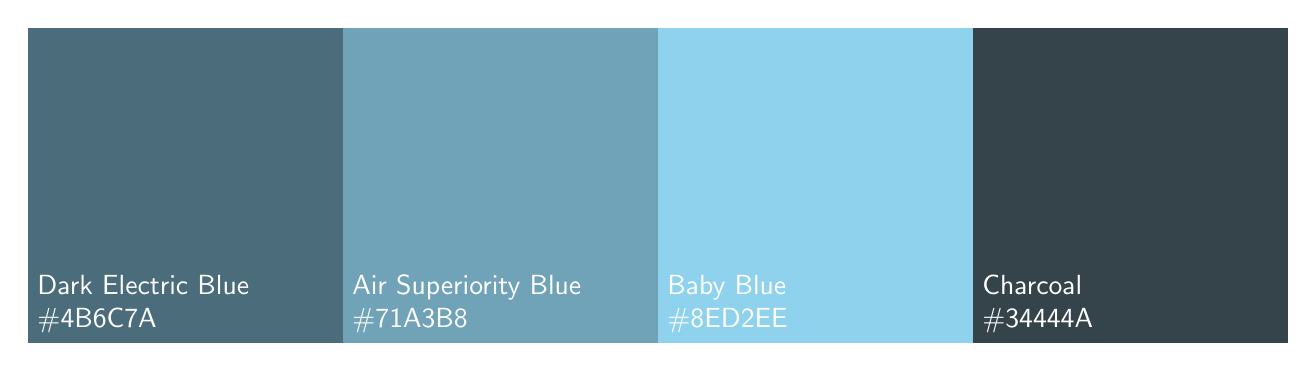
\begin{tikzpicture}[x=4cm,y=4cm]
\foreach \col/\name/\html/\textcol [count=\x] in {
	maincol1/Dark Electric Blue/4B6C7A/white,
	maincol2/Air Superiority Blue/71A3B8/white,
	maincol3/Baby Blue/8ED2EE/white,
	textcol/Charcoal/34444A/white%
	}{
	\fill[fill=\col] (\x,0) rectangle +(1,1);
	\node[align=left,anchor=south west,font=\sffamily,text=\textcol] at (\x,0) {\name\\\#\html};
	}
\end{tikzpicture}






%%% GRIJSPALET

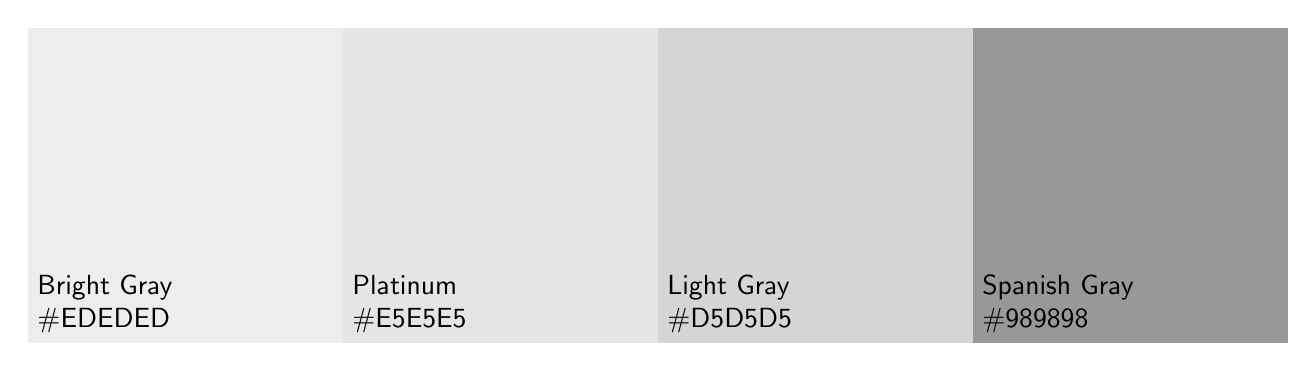
\begin{tikzpicture}[x=4cm,y=4cm]
\foreach \col/\name/\html/\textcol [count=\x] in {
	gray1/Bright Gray/EDEDED/black,
	gray2/Platinum/E5E5E5/black,
	gray3/Light Gray/D5D5D5/black,
	gray4/Spanish Gray/989898/black%
	}{
	\fill[fill=\col] (\x,0) rectangle +(1,1);
	\node[align=left,anchor=south west,font=\sffamily,text=\textcol] at (\x,0) {\name\\\#\html};
	}
\end{tikzpicture}





%%% SUBPALET 1

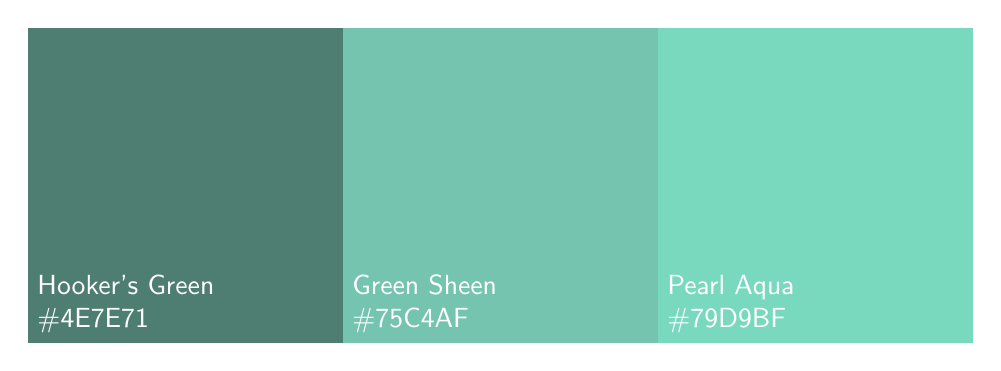
\begin{tikzpicture}[x=4cm,y=4cm]
\foreach \col/\name/\html/\textcol [count=\x] in {
	pal1col1/Hooker's Green/4E7E71/white,
	pal1col2/Green Sheen/75C4AF/white,
	pal1col3/Pearl Aqua/79D9BF/white%
	}{
	\fill[fill=\col] (\x,0) rectangle +(1,1);
	\node[align=left,anchor=south west,font=\sffamily,text=\textcol] at (\x,0) {\name\\\#\html};
	}
\end{tikzpicture}




%%% SUBPALET 2

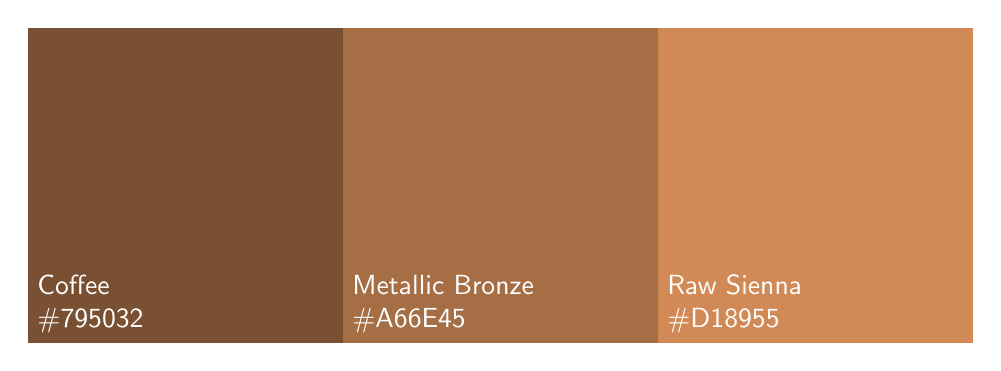
\begin{tikzpicture}[x=4cm,y=4cm]
\foreach \col/\name/\html/\textcol [count=\x] in {
	pal2col1/Coffee/795032/white,
	pal2col2/Metallic Bronze/A66E45/white,
	pal2col3/Raw Sienna/D18955/white%
	}{
	\fill[fill=\col] (\x,0) rectangle +(1,1);
	\node[align=left,anchor=south west,font=\sffamily,text=\textcol] at (\x,0) {\name\\\#\html};
	}
\end{tikzpicture}





%%% SUBPALET 3

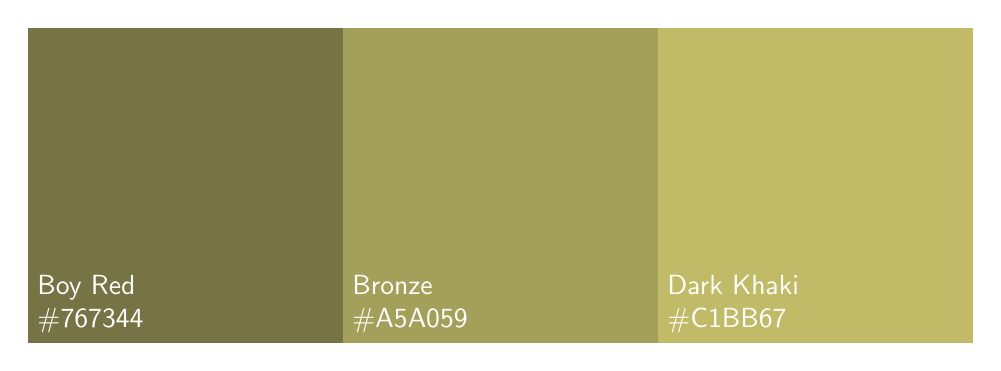
\begin{tikzpicture}[x=4cm,y=4cm]
\foreach \col/\name/\html/\textcol [count=\x] in {
	pal3col1/Boy Red/767344/white,
	pal3col2/Bronze/A5A059/white,
	pal3col3/Dark Khaki/C1BB67/white%
	}{
	\fill[fill=\col] (\x,0) rectangle +(1,1);
	\node[align=left,anchor=south west,font=\sffamily,text=\textcol] at (\x,0) {\name\\\#\html};
	}
\end{tikzpicture}






%%% unipolair


\begin{tikzpicture}[x=2cm,y=4cm]
\foreach \p [count=\x] in {20,40,60,80,100}{
	\fill[maincol1!\p] (\x,0) rectangle +(1,1);
	}
\draw[white,line width=5mm] (current bounding box.south west) rectangle (current bounding box.north east); 
\end{tikzpicture}



\begin{tikzpicture}[x=2cm,y=4cm]
\foreach \p [count=\x] in {20,36,52,68,84,100}{
	\fill[maincol1!\p] (\x,0) rectangle +(1,1);
	}
\draw[white,line width=5mm] (current bounding box.south west) rectangle (current bounding box.north east); 
\end{tikzpicture}



\begin{tikzpicture}[x=2cm,y=4cm]
\foreach \p [count=\x] in {20,31,43,54,66,77,89,100}{
	\fill[maincol1!\p] (\x,0) rectangle +(1,1);
	}
\draw[white,line width=5mm] (current bounding box.south west) rectangle (current bounding box.north east); 
\end{tikzpicture}





%%% bipolair



\begin{tikzpicture}[x=2cm,y=4cm]
\fill[gray1] (-.5,0) rectangle (.5,1);
\foreach \p [count=\x] in {50,100}{
	\fill[maincol2!\p!gray1] (\x,0) +(-.5,0)  rectangle +(.5,1);
	\fill[pal2col3!\p!gray1] (-\x,0) +(-.5,0)  rectangle +(.5,1);
	}
\draw[white,line width=5mm] (current bounding box.south west) rectangle (current bounding box.north east); 
\end{tikzpicture}



\begin{tikzpicture}[x=2cm,y=4cm]
\fill[gray1] (-.5,0) rectangle (.5,1);
\foreach \p [count=\x] in {33,66,100}{
	\fill[maincol2!\p!gray1] (\x,0) +(-.5,0)  rectangle +(.5,1);
	\fill[pal2col3!\p!gray1] (-\x,0) +(-.5,0)  rectangle +(.5,1);
	}
\draw[white,line width=5mm] (current bounding box.south west) rectangle (current bounding box.north east); 
\end{tikzpicture}







%%% nominaal








\end{document}

